\section{Discussion}
\subsection{Principal Findings and Interpretation of the Five-Mode Design}
In the primary C--E comparison, complete multi-channel configuration reduced mean completion time by 1.79 s (8.5\%; bootstrap 95\% CI, 1.10--2.51 s), and this direction was consistent across all operators and objects. The five-mode design distinguished the contribution of parameter configuration at three levels: C--D separated semantic display from parameter configuration, C--E compared the joint configuration of the master-side haptic and gripper-execution channels with impedance-only reconfiguration, and C--A and C--B provided fixed-parameter and manual-selection references, respectively. Because the two additional channels changed together, the C--E comparison was interpreted at the bundled system level.

The trajectory-length confidence interval included zero, and the two modes had the same median pause count (although the mean was lower in mode C). This pattern suggests that the time reduction may be associated with fewer corrective interruptions in some trials rather than shorter geometric paths; this process-level interpretation remains exploratory.
\begin{figure*}[t]
\centering
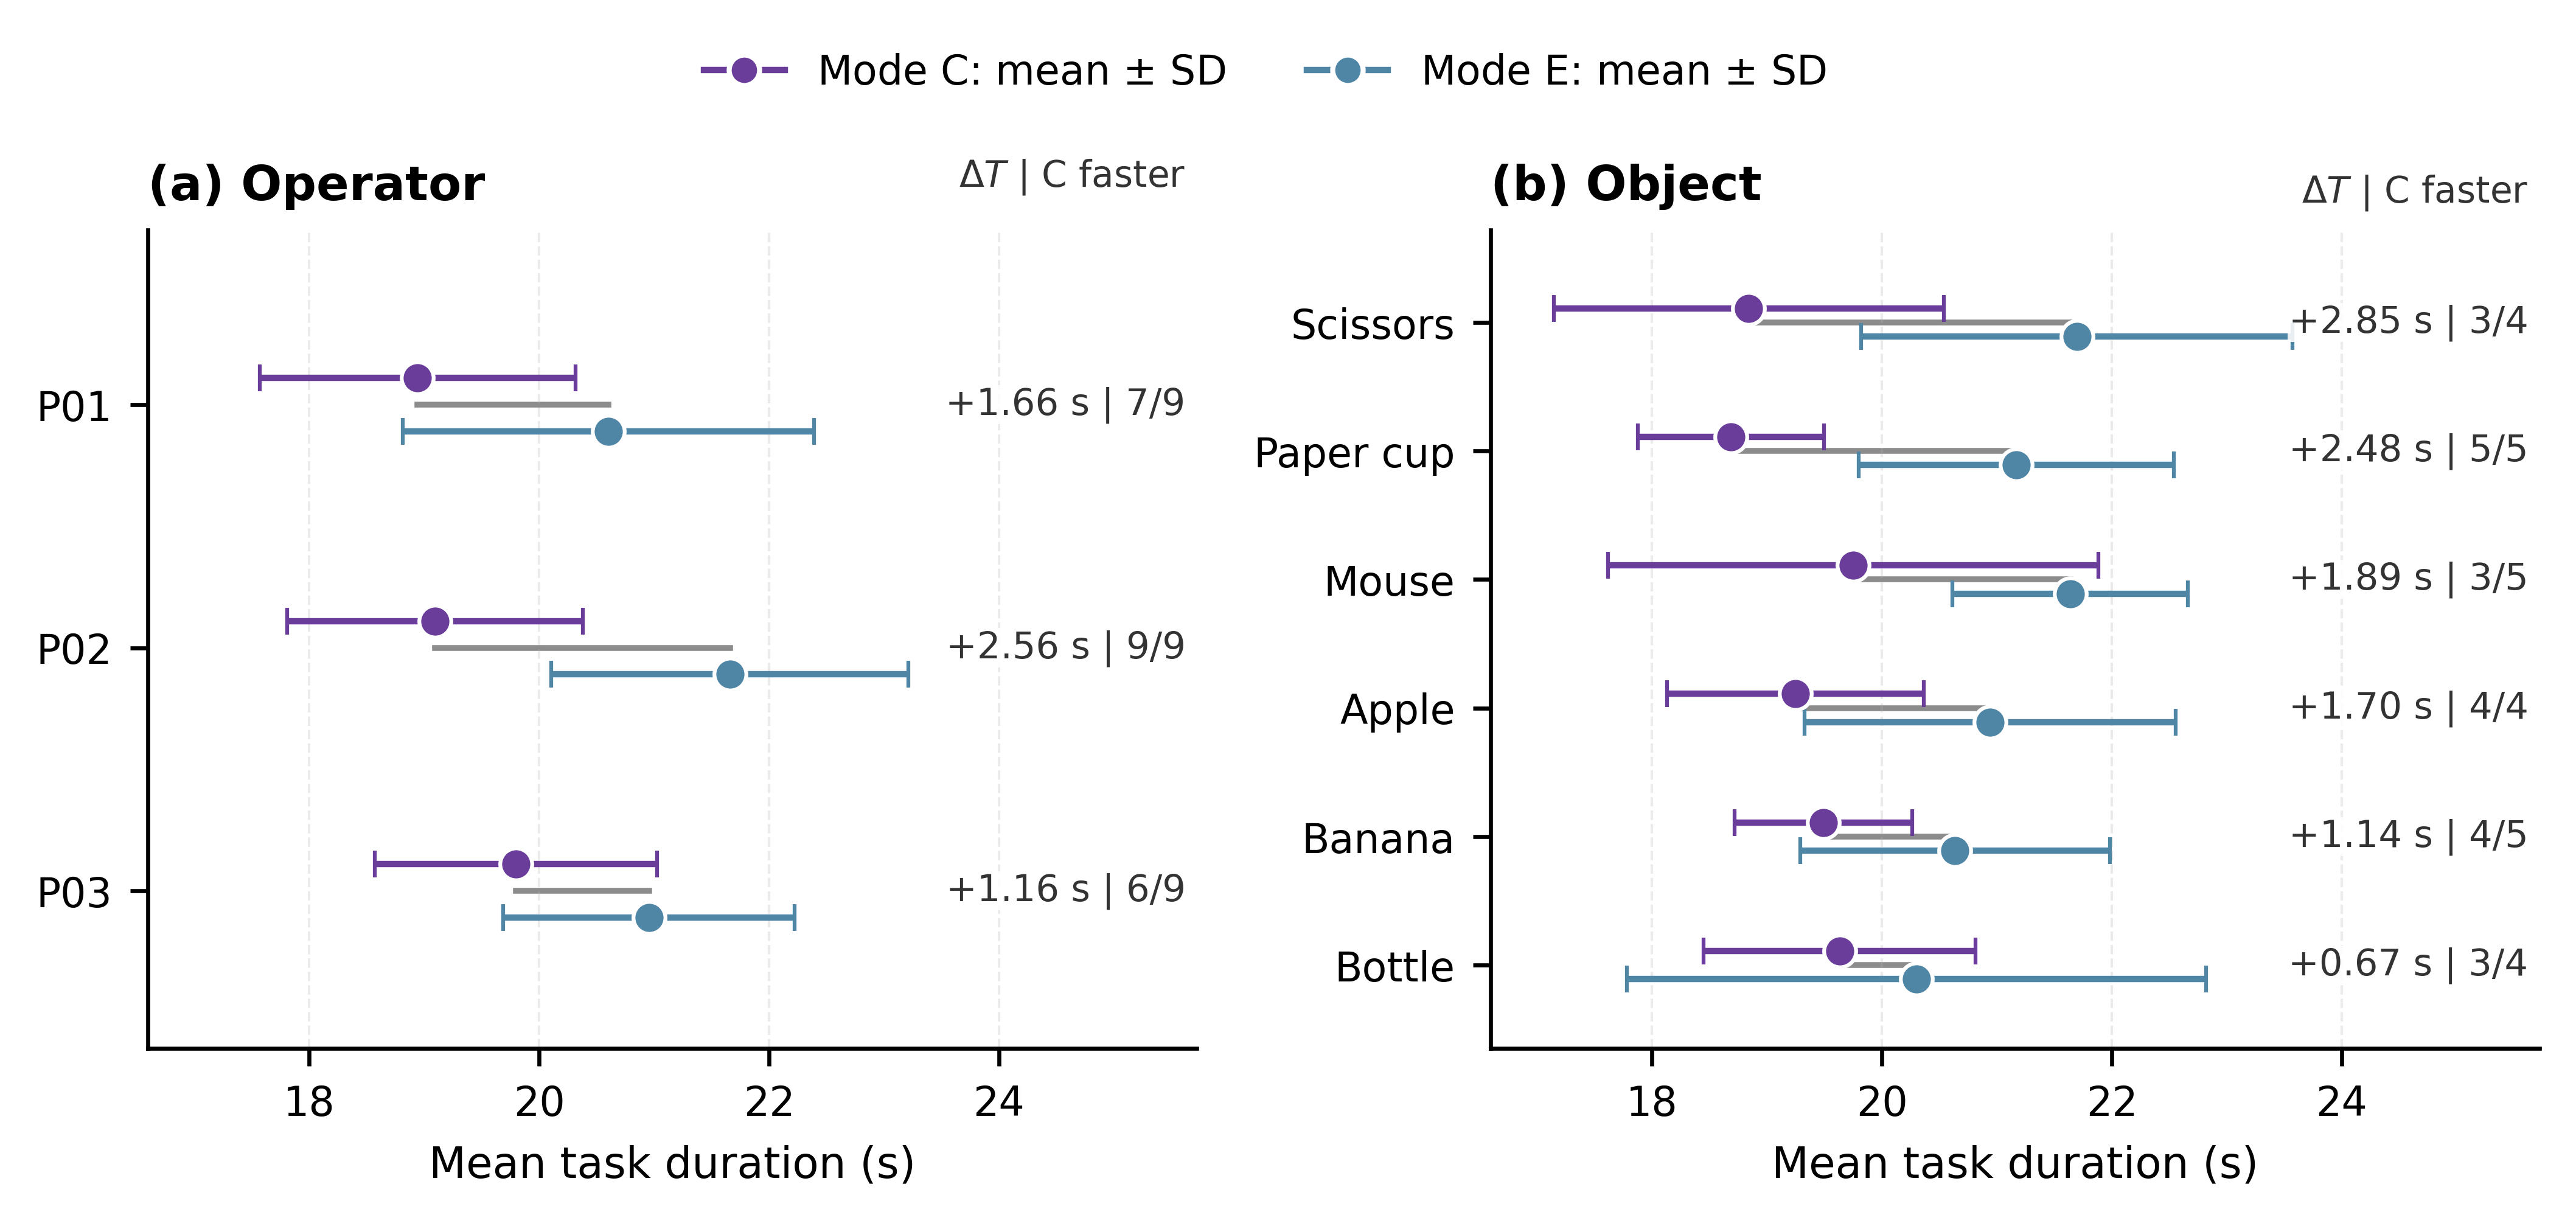
\includegraphics[width=\textwidth]{fig8.png}
\caption{Operator- and object-level summaries of task completion time for modes C and E. (a) Mean task completion time by operator ($n=9$ matched task blocks per operator). (b) Mean task completion time by object ($n=4$ or $5$ matched task blocks per object). Markers and horizontal error bars indicate mean $\pm$ SD for each mode. Right-side annotations report the mean paired difference ($\Delta T=T_E-T_C$) and the number of blocks in which mode C was faster divided by the total number of blocks. Positive $\Delta T$ values favor mode C. Error bars show within-group variability and are not confidence intervals for the paired differences.}
\label{fig:8}
\end{figure*}

\subsection{Asynchronous Perception--Control Integration}
Because visual output was used only for the one-shot strategy event, the perception process did not need to operate at the supervisory rate. Through bounded queues and non-blocking polling, the multi-rate architecture decoupled the 15-fps image stream and visual-inference process from the 200-Hz supervisory loop, placing semantic perception outside the high-rate critical path. The mean per-image processing time (48.19 ms) substantially exceeded one supervisory period (median, 5.07 ms), highlighting the importance of this decoupling. The architecture was designed for one-shot strategy configuration with subsequent locking; continuous visual servoing was outside the implemented control structure. Hard real-time guarantees and end-to-end trigger-to-contact timing remain uncharacterized.

\subsection{Variation Across Operators and Objects}
The positive mean C--E difference was consistent across all three operators and persisted in the leave-one-operator-out analyses (Fig.~\ref{fig:8}). Mode C also had a lower mean completion time than mode E for each of the six objects, with descriptive reductions ranging from 3.3\% (bottle) to 13.2\% (scissors). The larger reductions for the paper cup and scissors were consistent with the possibility that complete multi-channel configuration may be particularly valuable when deformation management or orientation retention is more demanding. Each object-level summary was based on four or five matched blocks and was therefore interpreted descriptively.

\subsection{Relation to Previous Work and Mechatronic Design Implications}
Prior tele-impedance and variable-impedance studies have adapted slave-side impedance using human-state information, contact-force information, demonstrations, or task phase \cite{ref06,ref07,ref08,ref09,ref18,ref19,ref20,ref21}. Vision-based methods have mapped object attributes, geometry, or vision--language representations to stiffness or impedance settings \cite{ref10,ref11,ref13,ref14}. Human-commanded stiffness interfaces can also exhibit coupling with force feedback in bilateral tele-impedance \cite{ref29}. Related work on automatic switching, shared control, multi-stiffness interfaces, and teleoperated grasping has addressed mode selection, control-authority allocation, and gripper impedance based on tactile deformation or grip-safety information \cite{ref12,ref15,ref16,ref23,ref24}.

The present framework complements these directions by using a single object-conditioned strategy event to coordinate a strategy-level operating state across slave-side impedance, master-side haptic feedback, and gripper execution. The principal contribution is therefore a cross-subsystem, strategy-level configuration architecture together with a system-level evaluation of the resulting multi-channel coordination. At the software-architecture level, bounded queues, non-blocking polling, one-shot triggering, and strategy locking decouple low-rate semantic perception from the nominal 200-Hz supervisory execution path and prevent repeated parameter switching within a trial.

This design principle may be useful in semi-structured applications such as flexible sorting, remote maintenance, and dismantling, where a limited set of recurring object or task classes can be associated with predefined and experimentally screened operating strategies. Extending the framework to larger class sets would require systematic maintenance of the object-class-to-strategy mapping and may require a richer strategy space than the three levels evaluated here. Tactile or contact-state sensing could be added as a post-contact verification layer, enabling corrective updates after contact without requiring the visual process to operate within the nominal 200-Hz supervisory execution path.
\subsection{Scope and Future Extensions}
The experimental evidence was obtained from three operators, six known objects, translational master motion, a fixed end-effector orientation, prescribed object placement, and preassigned mode orders without complete counterbalancing. The class-to-strategy mapping was manually defined. The findings therefore characterize the present platform and task within the tested sample.

Several measurement and design limitations should be considered in future work. First, because the C--E contrast changed the master-side haptic and gripper-execution channels together, separate channel-level ablations are required to resolve their individual contributions. Second, the trial logs did not retain event-level object-class labels, confidence scores, or synchronized strategy-event/contact timestamps; trial-level verification of online trigger timing requires synchronized visual, strategy-event, and contact logging. Third, outcome labels were based on direct observation without independent video-based re-rating. Fourth, although smoothstep interpolation was used for impedance transitions, no formal transient-stability analysis of the complete teleoperation system was performed. Finally, the retained haptic data characterize the commanded signal but not the realized device output, and no saturation-status signal was recorded. Future experiments should combine synchronized logging, independent video-based outcome assessment, formal stability analysis, direct measurements of contact and realized haptic output, saturation monitoring, and systematic parameter optimization.
